\begin{quote}
Things in motion sooner catch the eye\\
Than what not stirs.\\
--W.S., ``Troilus and Cressida'' 
\end{quote}

The Elliptic Billiard (EB) consists of a particle moving with constant velocity in the interior of an ellipse, bouncing elastically against its boundary. A few trajectory regimes are shown in Figure~\ref{fig:billiard-trajectories}. Though the EB has been exhaustively studied \cite{dragovic11,sergei91}, can it still yield any surprises?

\begin{figure}
    \centering
    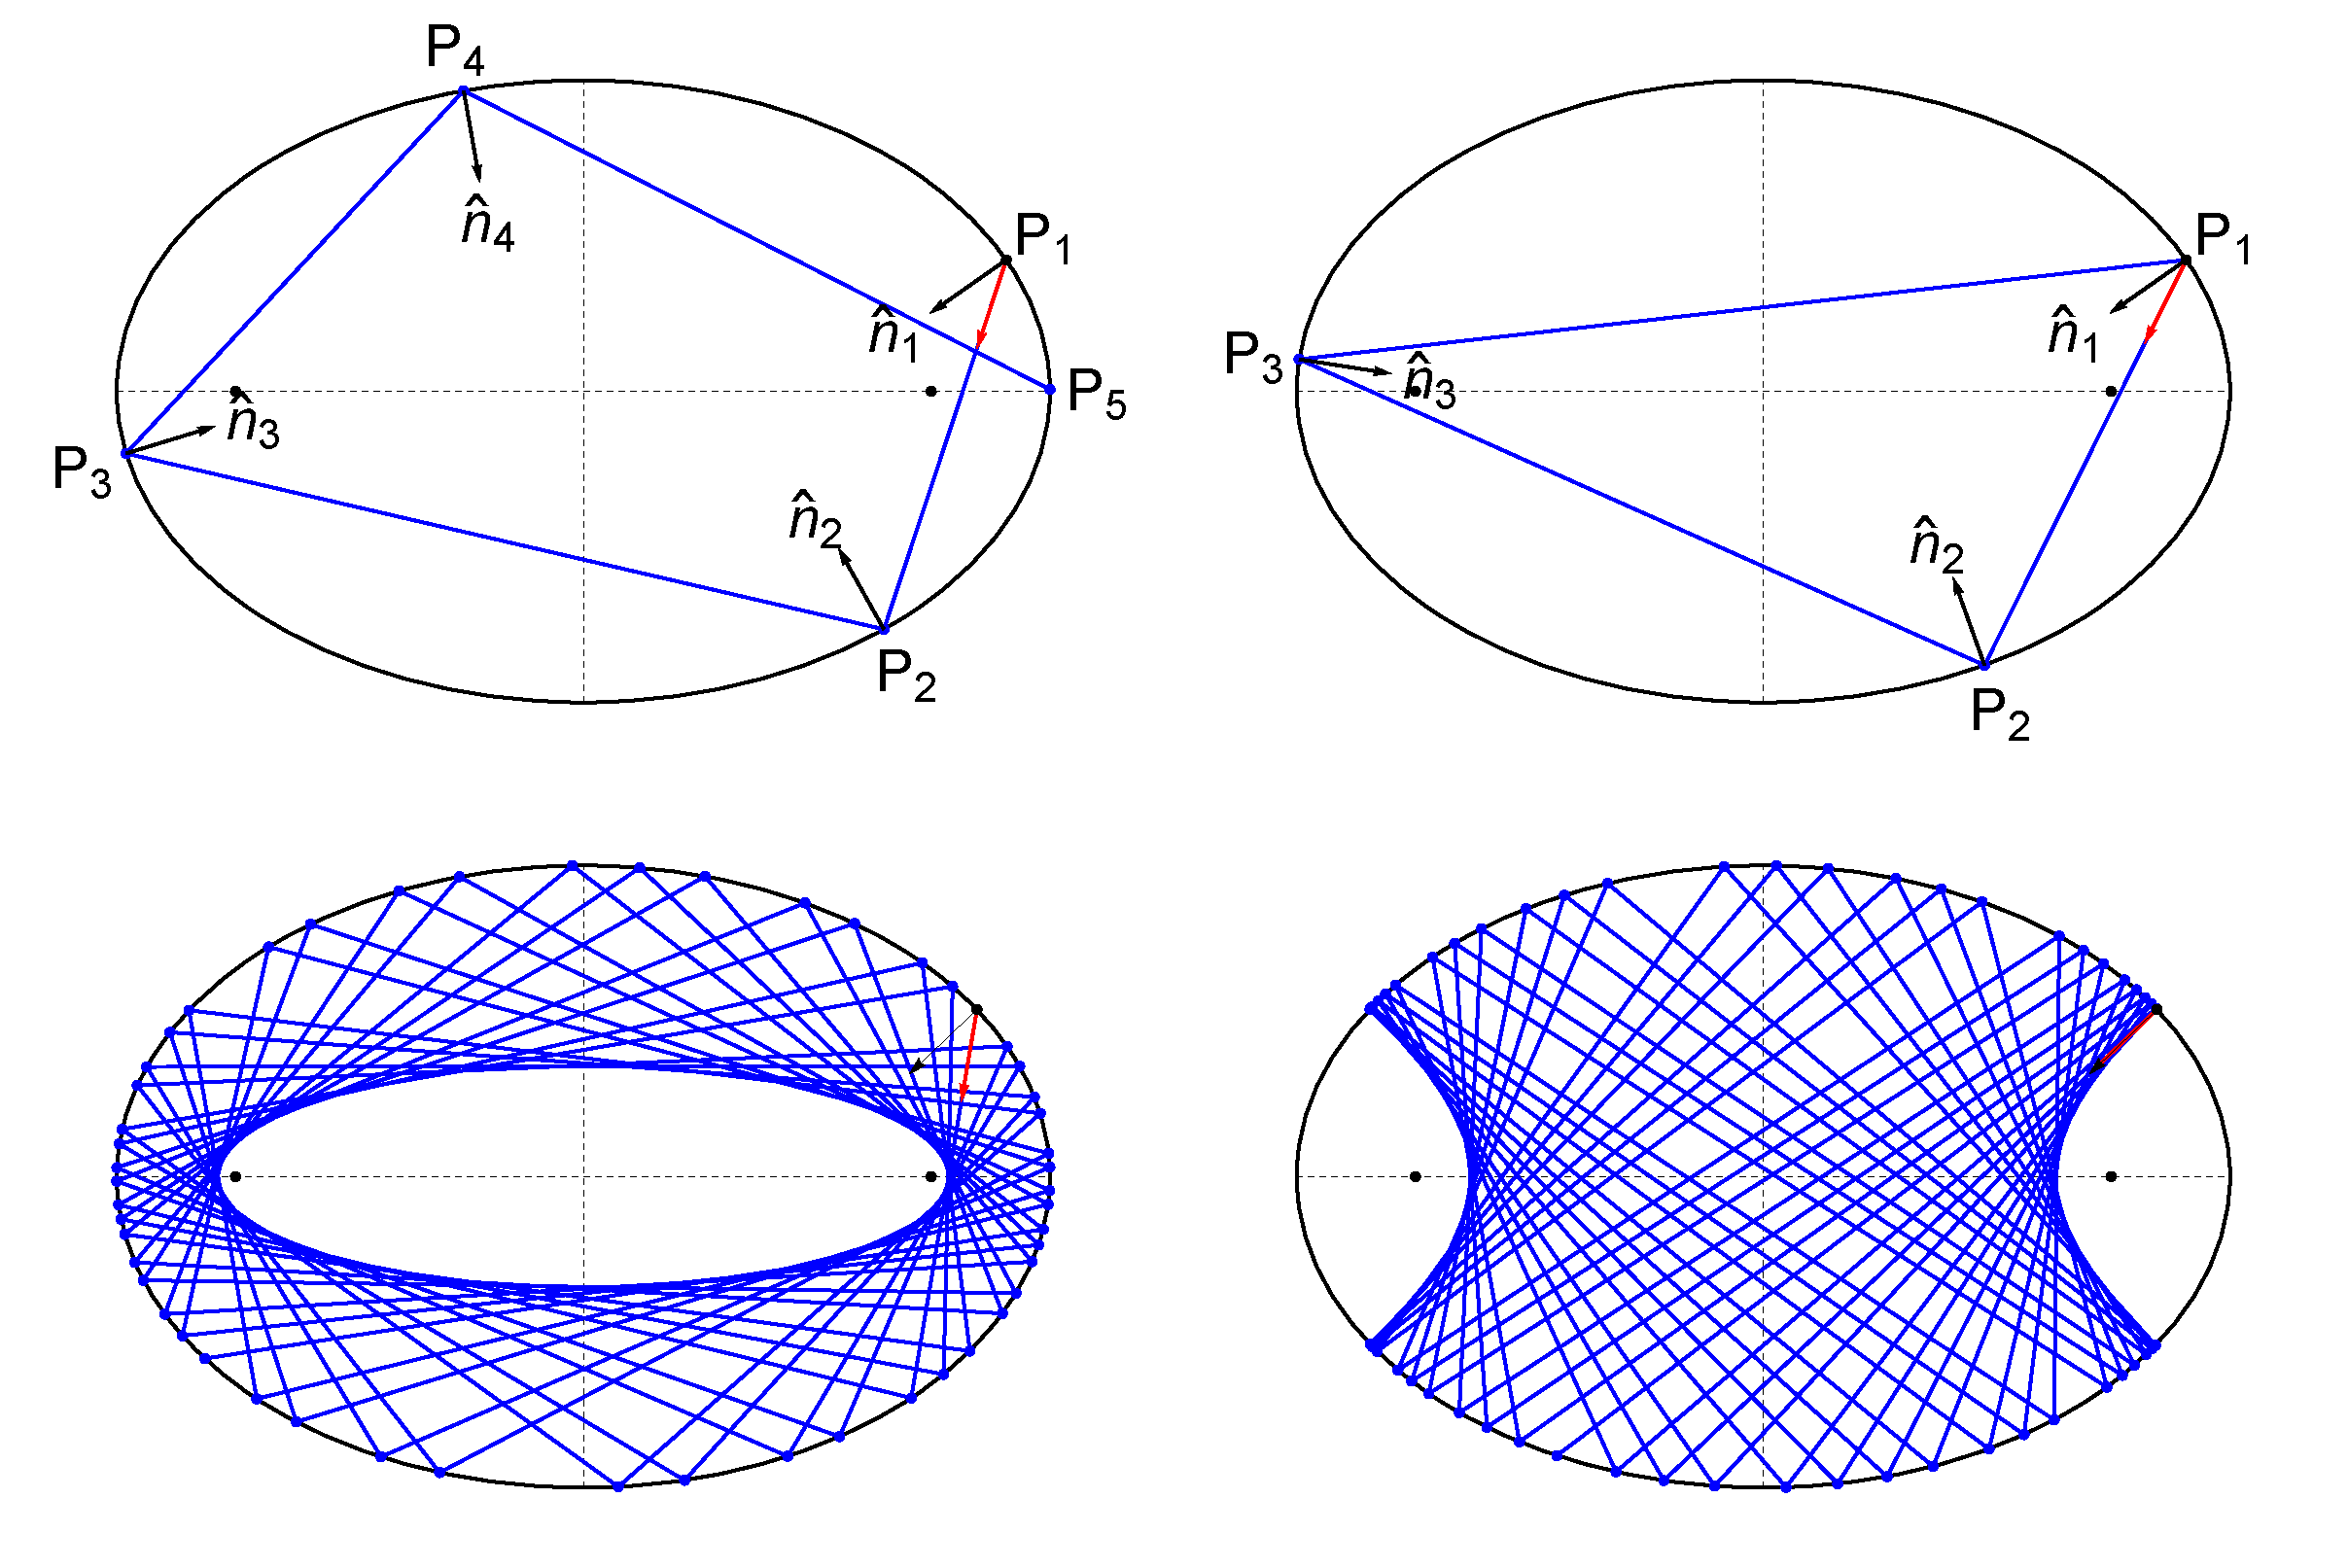
\includegraphics[width=\textwidth]{pics/u1000_billiard_trajectories.pdf}
    \caption{Particle trajectories in an Elliptic Billiard. \textbf{Top left}: the first four segments of a trajectory starting at $P_1$ along the red arrow, bouncing elastically at $P_2$ (reflecting about normals $\hat{n}_i$), etc. \textbf{Top right}: a 3-periodic trajectory. \textbf{Bottom}: quasi-periodic regimes tangent to an elliptic (left) or hyperbolic (right) {\em Caustic}. The first (resp. second) regime is established if a segment passes outside (resp. between) the foci (black dots).
    % done
    \href{https://youtu.be/A7mPzrNJHkA}{Video} \cite[pl\#1]{dsr_math_intell_playlist}}
    \label{fig:billiard-trajectories}
\end{figure}

In 2011, we uploaded a
% done
\href{https://www.youtube.com/watch?v=9xU6T7hQMzs}{video} \cite[pl\#2]{dsr_math_intell_playlist} showing the family of 3-periodic trajectories as a continuous set of rotating triangles. We also drew the locus of their Incenter and {\em Intouchpoints}\footnote{Where the Incircle touches a triangle's sides}. Though the latter was a self-intersecting sextic, Figure~\ref{fig:intro-plot}, we were surprised the former was (numerically) a perfect ellipse. For a refresher on triangle concepts see Figure~\ref{fig:constructions}. 

\begin{figure}
    \centering
    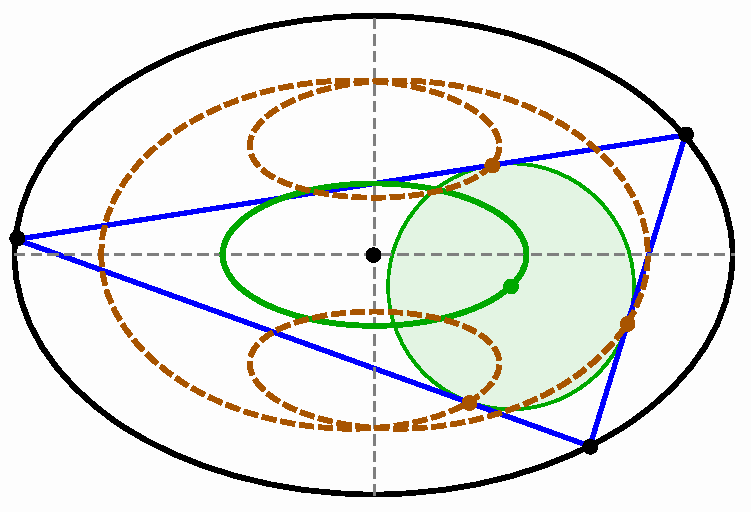
\includegraphics[width=.7\textwidth]{pics/u1001_intro_plot.pdf}
    \caption{An $N=3$ orbit (blue), its Incircle (transparent green), Incenter (green dot) and Intouch Points (brown dots). Over the $N=3$ family, the Incenter locus is a perfect ellipse (green), while the Intouchpoints produce a self-intersecting sextic (dashed brown).
    % done
    \href{https://youtu.be/9xU6T7hQMzs}{Video} \cite[pl\#2]{dsr_math_intell_playlist}}
    \label{fig:intro-plot}
\end{figure}
%
 Over the next few years there surfaced elegant proofs showing that the locus of the Incenter \cite{ronaldo16,olga14}, Barycenter \cite{ronaldo19,sergei2016}, Circumcenter  \cite{corentin19,ronaldo19}, and Orthocenter \cite{ronaldo19} were all ellipses. Such a stream of results ushered us, some eight years later, into this second exploratory cycle. Never could we anticipate the surprises still in store!

\begin{figure}
    \centering
    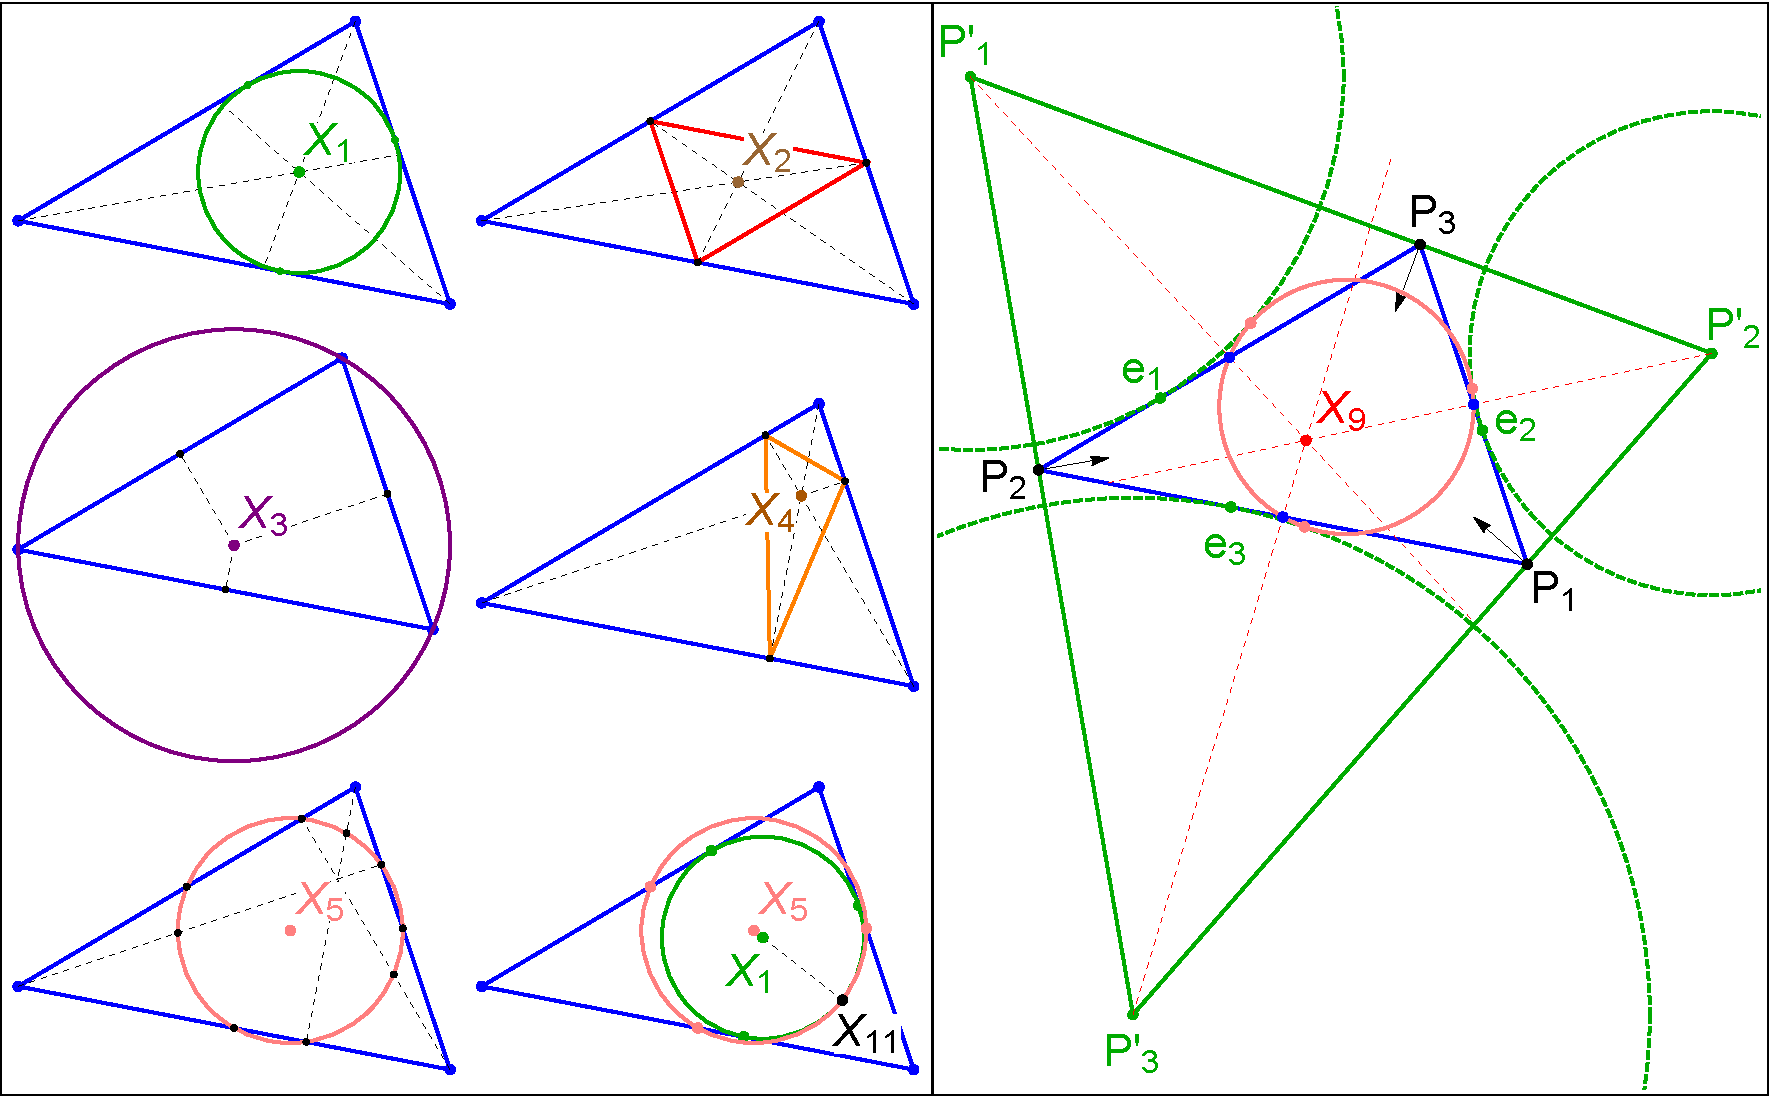
\includegraphics[width=\textwidth]{pics/u0039_constr.pdf}
    \caption{Notable Triangle Points, referred to as $X_i$, after Kimberling \cite{etc}. \textbf{Left}: The Incenter $X_1$ is the intersection of angular bisectors, and center of the Incircle (green), a circle tangent to the sides at three {\em Intouchpoints} (green dots), its radius is the {\em Inradius} $r$. The Barycenter $X_2$ is where lines drawn from the vertices to opposite sides' midpoints meet. Side midpoints define the {\em Medial Triangle} (red). The Circumcenter $X_3$ is the intersection of perpendicular bisectors, the center of the {\em Circumcircle} (purple) whose radius is the {\em Circumradius} $R$. The Orthocenter $X_4$ is where altitudes concur. Their feet define the {\em Orthic Triangle} (orange). $X_5$ is the center of the 9-Point (or Euler) Circle (pink): it passes through each side's midpoint, altitude feet, and Euler Points \cite{mw}. The Feuerbach Point $X_{11}$ is the single point of contact between the Incircle and the 9-Point Circle. \textbf{Right}: given a reference triangle $P_1P_2P_3$ (blue), the {\em Excenters} $P_1'P_2'P_3'$ are pairwise intersections of lines through the $P_i$ and perpendicular to the bisectors. This triad defines the {\em Excentral Triangle} (green). The {\em Excircles}  (dashed green) are centered on the Excenters and are tangent to the triangle sides at the {\em Extouch Points} $e_i,i=1,2,3$. Lines drawn from each Excenter through sides' midpoints (dashed red) concur at the {\em Mittenpunkt} $X_9$. Also shown is Feuerbach's Theorem \cite{mw}: besides the Incircle, the 9-Pt Circle (pink) touches each Excircle at a single point (pink dots), the vertices of the {\em Feuerbach Triangle}.}
    \label{fig:constructions}
\end{figure}

\begin{figure}
    \centering
    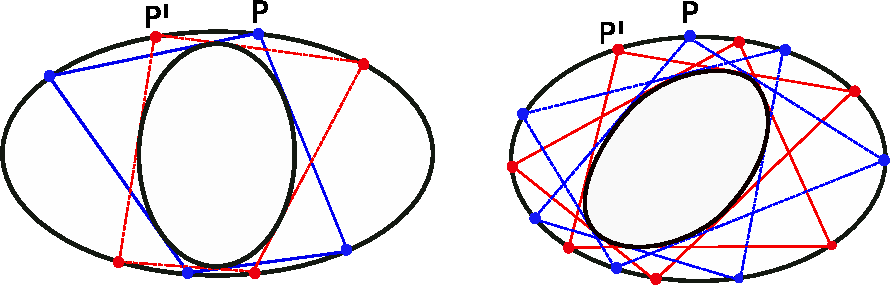
\includegraphics[width=1.0\textwidth]{pics/u0003_poncelet_porism.pdf}
    \caption{Poncelet's Porism states that given two nested ellipses, if one closed trajectory with $N$ sides can be found starting at a point $P$ on the boundary of the outer
while remaining tangent to the inner, then every boundary point (e.g., $P'$) can initiate an $N$-trajectory, i.e., there exists a one-dimensional {\em family} of closed trajectories.}
\label{fig:poncelet-porism}
\end{figure}

\subsection{An experimental approach and an unexpected breakthrough}

Keen to examine the loci of other {\em Triangle Centers}\footnote{A point defined in terms of vertex positions and angles which is invariant with respect to rigid transformations.} over the $N=3$ orbit family\footnote{Here we also use $N=3$, $N=4$ to denote 3-periodic, 4-periodic, etc.}, we built an interactive \href{https://editor.p5js.org/undefined/present/i1Lin7lt7}{applet} \cite{dsr_applet_x12345}. We started with the first 100 centers catalogued on Clark Kimberling's Encyclopedia\footnote{More than 40,000 are listed there!} \cite{etc}. The loci these produced were quite entertaining: ellipses, circles, a stationary point, a quartic, one with kinks, etc., see our \href{https://dan-reznik.github.io/Elliptical-Billiards-Triangular-Orbits/loci_6tri.html}{locus gallery} \cite{reznik_media}. Interestingly, a few ellipses were similar and/or identical to the Billiard or its Caustic \cite{reznik2020-loci}. 

Beyond loci, the $N=3$ family revealed an amazing property: the ratio of Inradius to Circumradius is %\ldots{ } 
invariant. Right under our noses, we thought!
In turn, this immediately dictated surprising relations involving orbit angles and areas.

At this point a remarkable object steps in, coaxing us into a breakthrough: Monge's Orthoptic Circle,  Figure~\ref{fig:monge-orthoptic}. Its direct connection with the $N=4$ family has been explored by eminent mathematicians \cite{connes07}. Close observation of its geometry provided a bridge with which to generalize $N=3$ invariants to orbits of any $N$. Indeed, there exist generic constructions for point, circular and Caustic loci which are analogous to the $N=3$ case. Additionally, conservation of angular and area quantities already verified in $N=3$ hold true for all $N$. Having started this exploration with the humble triangle, these were remarkable surprises. Merci, Gaspard!

%The flow of our investigations is summarized in %Figure~\ref{fig:global-diagram}.
%
\begin{figure}[ht]
    \centering
    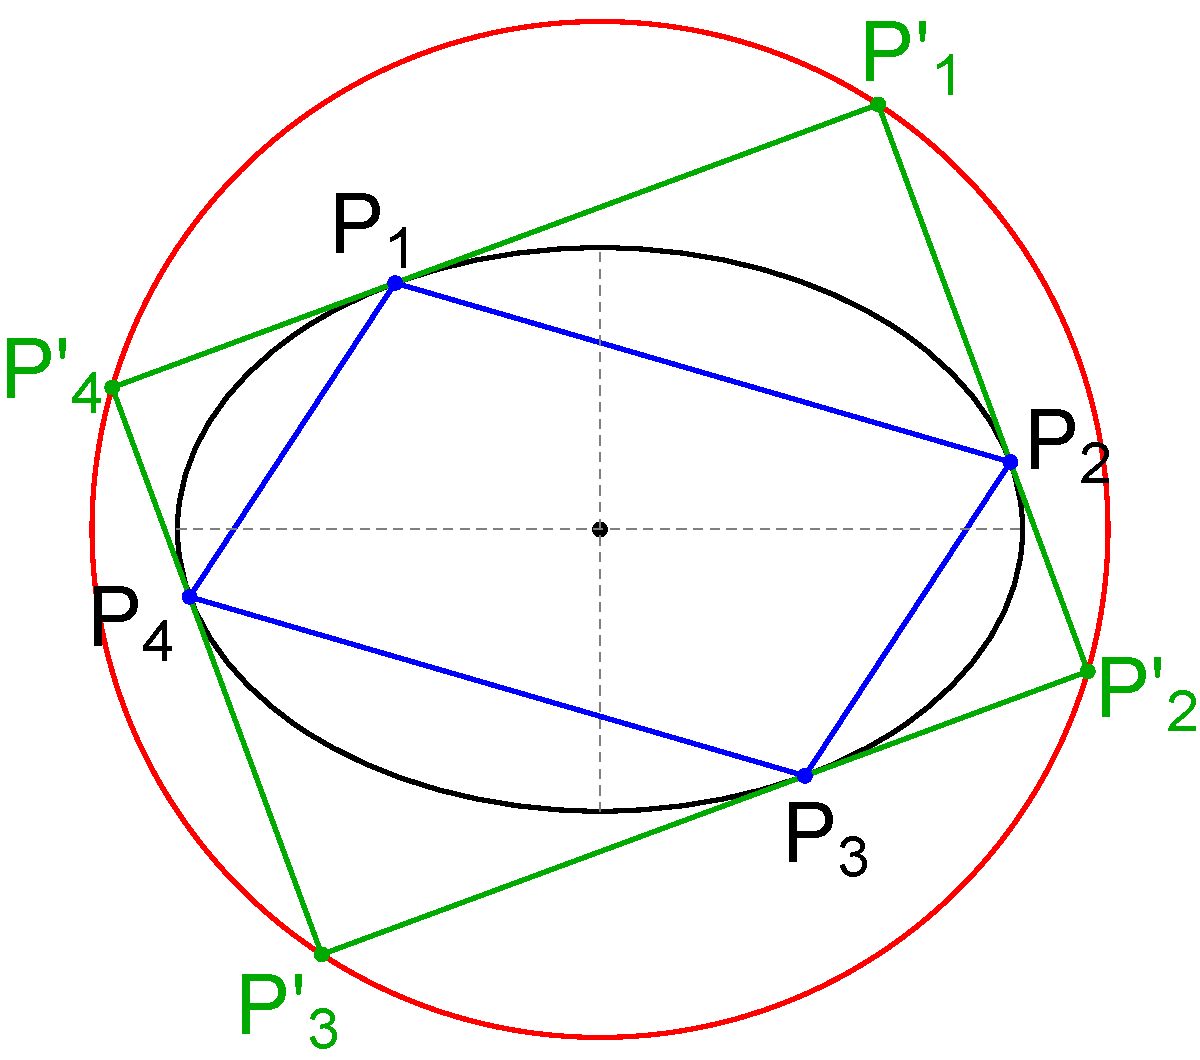
\includegraphics[width=.5\textwidth]{pics/u0200_monge_orthoptic.pdf}
    \caption{Gaspard Monge (1746--1818) discovered that the locus of points whose tangents to a given ellipse subtend a right angle is a circle (red), called the {\em Orthoptic} Circle. Its connection with Billiards is remarkable \cite{connes07}: From a point $P_1'$ on the circle, shoot two rays tangent to the ellipse, intersecting them with the circle at $P_2'$ and $P_4'$. From either one shoot one new tangent ray and obtain $P_3'$. Four surprises: (i) the intersections form a rectangle (green); (ii) the points of tangency with the ellipse define a parallelogram (blue), which is (iii) a billiard orbit of the ellipse; (iv) all $N=4$ non-intersecting orbits are constant perimeter parallelograms. 
    \href{https://youtu.be/9fI3iM2jrmI}{Video} \cite[pl\#5]{dsr_math_intell_playlist}}    \label{fig:monge-orthoptic}
\end{figure}

As we crossed over to $N>3$, our analytical methods became insufficient. Luckily we were helped by generous mathematicians who contributed insights and proofs \cite{akopyan19_private_meromorphic,helman19,dominique19,olga19_mitten,sergei19_private_circles,sergei19_private_meromorphic}, see Acknowledgements and \cite{sergei2020}. 

We challenge the reader with some questions in the Conclusion and very much welcome feedback. Many of our experiments are available as videos on a YouTube \href{https://bit.ly/2kTvPPr}{playlist} \cite{dsr_math_intell_playlist}. In the text, these are cited as {[n,~pl\#m]}, where n is the standard reference number and m is the video entry into the playlist. Section~\ref{sec:list-videos} provides a quick-reference and links to all videos mentioned below.